\section{Zbiór danych}
\label{sec:dane}

W~projekcie wykorzystane zostaną dane ze zbioru \emph{FIFA 19 Complete Player Dataset}~\cite{fifa-dataset} z~serwisu \url{kaggle.com}.


\subsection{Charakterystka zbioru danych}
\label{subsec:charakterystka}
Każdy zawodnik ze zbioru danych posiada ponad 70 użytecznych atrybutów opisujących jego umiejętności gry w~piłkę nożną. Wśród nich znajdują się atrybuty opisujące m.in. kontrolę piłki, przyspieszenie czy celność strzałów z~dystansu. 

Większość atrybutów jest opisana za pomocą wartości całkowitych z~zakresu $[0, 99]$. Niektóre atrybuty zostały opisane liczbą całkowitą z~zakresu $[0,5]$. W~zestawie danych, pojawiły się atrybuty ciągłe opisujące wartość zawodnika, jego tygodniówkę, wzrost, wiek i~wagę oraz atrybuty kategoryczne opisujące preferowaną nogę (lewa lub prawa), typ budowy ciała oraz jego główną pozycję.

Każdemu zawodnikowi przypisany jest atrybut kategoryczny opisujący główną pozycję na boisku oraz 26 wskaźników numerycznych, określających jak dobry jest dany zawodnik na poszczególnych pozycjach.

Dodatkowo, zbiór danych został uzupełniony o~metadane opisujące samego zawodnika, takie jak numer na koszulce, nazwisko, link do zdjęcia, drużyna, narodowość czy międzynarodową reputację. 

\begin{figure}[t]
    \centering    
    \begin{tabular}{cc}
    \subfloat[\emph{Short Passing}]{
        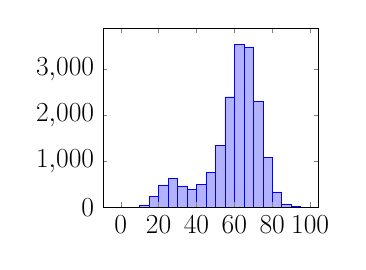
\begin{tikzpicture}[thick, scale=0.4]
            \Huge
            \begin{axis}[ymin=0, area style]
                \addplot+[ybar interval,mark=no] plot coordinates { (0, 0) (5, 3) (10, 53) (15, 242) (20, 485) (25, 632) (30, 465) (35, 397) (40, 503) (45, 766) (50, 1350) (55, 2408) (60, 3553) (65, 3496) (70, 2309) (75, 1084) (80, 336) (85, 65) (90, 12) (95, 0) };
            \end{axis}
        \end{tikzpicture}
    } &
    \subfloat[\emph{Strength}]{
        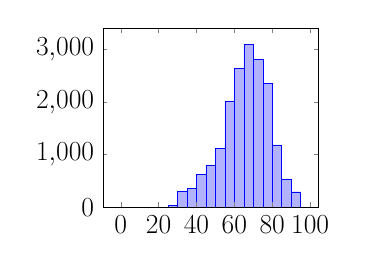
\begin{tikzpicture}[thick, scale=0.4]
            \Huge
            \begin{axis}[ymin=0, area style]
                \addplot+[ybar interval,mark=no] plot coordinates { (0, 0) (5, 0) (10, 0) (15, 1) (20, 2) (25, 40) (30, 301) (35, 354) (40, 618) (45, 800) (50, 1121) (55, 2015) (60, 2631) (65, 3093) (70, 2810) (75, 2354) (80, 1182) (85, 539) (90, 294) (95, 4) };
            \end{axis}
        \end{tikzpicture}    
    } \\
    \subfloat[\emph{Agility}]{
        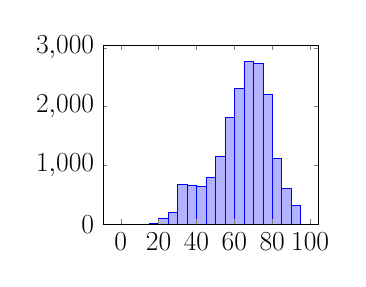
\begin{tikzpicture}[thick, scale=0.4]
            \Huge
            \begin{axis}[ymin=0, area style]
                \addplot+[ybar interval,mark=no] plot coordinates { (0, 0) (5, 0) (10, 1) (15, 11) (20, 108) (25, 201) (30, 682) (35, 667) (40, 639) (45, 805) (50, 1156) (55, 1813) (60, 2308) (65, 2770) (70, 2734) (75, 2216) (80, 1116) (85, 607) (90, 320) (95, 5) };
            \end{axis}
        \end{tikzpicture}
    } &
    \subfloat[\emph{GK Positioning}]{
        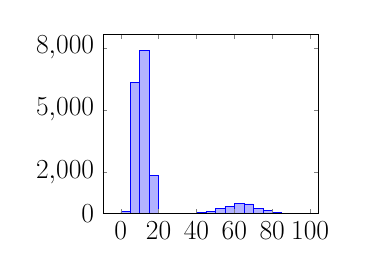
\begin{tikzpicture}[thick, scale=0.4]
            \Huge
            \begin{axis}[ymin=0, area style, ytick={0, 2000, 5000, 8000}]
                \addplot+[ybar interval, mark=no] plot coordinates { (0, 81) (5, 6337) (10, 7876) (15, 1831) (20, 4) (25, 1) (30, 3) (35, 3) (40, 31) (45, 88) (50, 227) (55, 326) (60, 460) (65, 450) (70, 251) (75, 127) (80, 51) (85, 11) (90, 1) (95, 0) };
            \end{axis}
        \end{tikzpicture}
    } \\

    \end{tabular}
    \caption{Przykładowe rozkłady wartości atrybutów z~podanego zbioru danych}
    \label{fig:rozklady-atrybutow}
\end{figure}

Na rysunku~\ref{fig:rozklady-atrybutow} zostały zaprezentowane przykładowe rozkłady wartości badanych atrybutów. W~głównej mierze, są to rozkłady normalne lub gruboogonowe. Ciekawy rozkład mają atrybuty opisujące umiejętności bramkarskie. Z~racji nietypowej specyfiki tej pozycji, atrybuty te mają rozkład dwumodalny. Wysoki lewy pik rozkładu opisuje zawodników z~pola, których umiejętności bramkarskie są niewielkie ale jest ich zdecydowanie więcej. Prawy niewielki pik opisuje rzeczywistych bramkarzy, którzy mają niewątpliwie większe umiejętności, jednak jest ich wyraźnie mniej. Obecność bramkarzy w~zestawie danych jest również jednym z~powodów dla którego część rozkładów ma gruby ogon po lewej stronie. 

\subsection{Przygotowanie atrybutów}
\label{subsec:atrybuty}
\emph{Implementacja ładowania, wstępnego przetwarzania danych oraz selekcji atrybutów została umieszczona w~pliku \texttt{data-preparation.R}} \\

W~pierwszej kolejności, z~racji niewielkiej liczby brakujących wartości, usunęliśmy wszystkie przykłady, które nie posiadały wszystkich wypełnionych kolumn. Ze zbioru należy usunięte zostały atrybuty opisowe, określające nieinteresujące cechy takie jak narodowość, aktualna drużyna, reputacja na świecie czy imię oraz nazwisko. Dodatkowo, ze zbioru danych zostały usunięte atrybuty opisujące numeryczną wartość opisującą umiejętność gry danego zawodnika na danej pozycji. Informacja tego typu znacząco upraszcza zadanie, sprowadzając zadanie do wyboru najwyższej wartości z~podanego zbioru. 

W kolejnym kroku, atrybuty nominalne, niosące ze sobą pewną informację należało sprowadzić do postaci numerycznej. Atrybut binary \emph{Preferred.Foot} został zamieniony na wartość liczbową ze zbioru $[0,1]$. Atrybut \emph{Work.Rate}, opisujący zaangażowanie danego zawodnika w~grę w~ataku oraz w~obronie, posiadał dziewięć nominalnych wartości, takich jak: \texttt{Low/ Medium}, \texttt{High/ Low}, \texttt{High/ High} itp.. Zdecydowaliśmy się rozbić ten atrybut na dwa atrybuty porządkowe \emph{Work.Rate.Offensive} oraz \emph{Work.Rate.Defensive}, które mogły przyjmować wartości $[$\texttt{Low}, \texttt{Medium}, \texttt{High} $]$. Ostatecznie, wartości te zostały sprowadzone do wartości numerycznych, za pomocą polecenia \texttt{as.numeric}.

Kolejnym rozważanym atrybutem, był \emph{Body.Type}. Pierwotnie, posiadał on dziesięć różnych wartości, jednak po zagłębieniu się w~zbiór danych, okazało się że siedem z~nich to wartości unikalne w~całym zbiorze. Wynikają one ze specyfiki gry, w~której wyróżniające się postacie (np. Lionel Messi czy Cristiano Ronaldo), otrzymały własny model postaci. Zgodnie z~wiedzą ekspercką, zminimalizowliśmy zbiór wartości do trzech wartości nominalnych $[$\texttt{Lean}, \texttt{Normal}, \texttt{Stocky}$]$, które ostatecznie również zamieniliśmy na wartości numeryczne. 

Następnym krokiem we~wstępnym przetwarzaniu była konwersja wzrostu (zapisanego w~stopach) na metry oraz wagi (zapisanej w~funtach) na kilogramy oraz policzenie grupującego wskaźnika \emph{Body-Mass Index}. Ostatecznie, każdy z~przygotowanych atrybutów został przeskalowany w~taki sposób, aby jego średnia wartość wynosiła~$0$, a~odchylenie standardowe było równe~$1$. W~ten sposób, otrzymaliśmy obiekt typu \emph{data frame} zawierający $45$ zmiennych oraz $18159$ przykładów.

Jako atrybut ukryty, potraktowana zostania optymalna pozycja na boisku. W~celu przeprowadzenia analizy poprawności badanego algorytmu grupowania, zakładamy że pozycja na boisku zapisana w~zbiorze danych jest jego rzeczywistą optymalną pozycją. Atrybut ten jest niezwykle ciekawy do analizy, ponieważ można go analizować na trzech poziomach:

\begin{itemize}
    \item na podstawie gry w~polu:
        \begin{itemize}
            \item bramkarz,
            \item zawodnik z~pola,
        \end{itemize}
    \item na podstawie ogólnej pozycji:
        \begin{itemize}
            \item bramkarz,
            \item obrońca,
            \item pomocnik,
            \item napastnik,
        \end{itemize}
    \item na podstawie szczegółowej pozycji:
    \begin{itemize}
        \item bramkarz,
        \item środkowy obrońca, 
        \item lewy/prawy boczny obrońca
        \item lewy/prawy wahadłowy,
        \item pomocnik ofensywny,
        \item lewy/środkowy/prawy pomocnik,
        \item pomocnik defensywny,
        \item napastnik,
        \item lewy/prawy skrzydłowy.
    \end{itemize}
\end{itemize}

Oprócz tego, w~zależności od wyników grupowania, można spróbować zdefiniować bardziej wyrafinowane pozycje m.in.: 
\emph{mezzala}, \emph{mediano}, \emph{trequartista} czy libero.

\subsection{Wstępne ograniczenie liczby atrybutów}
\label{subsec:ograniczanie-atrybtow}
W~celu skrócenia czasu obliczeń oraz wyeliminowania niepewności związanej z~za dużą liczbą zmiennych, zdecydowaliśmy się ograniczyć liczbę atrybutów z~$45$ do~$20$. Liczba ta została określona na podstawie macierzy korelacji atrybutów. Na jej podstawie, wybraliśmy zestawy atrybutów, które połączyliśmy ze sobą poprzez policzenie ich średnich arytmetycznych. Tak skonstruowane atrybuty zostały przedstawione w~tabeli~\ref{tab:nowe-atrybuty}.

\begin{table}[h]
\centering
\begin{tabular}{|c|l|}
\hline
\textbf{Nowy atrybut} & \multicolumn{1}{c|}{\textbf{Atrybuty pierwotne}}                  \\ \hline
GK.Skills             & \multicolumn{1}{p{5cm}|}{\raggedright GKDiving, GKHandling, GKKicking, GKPositioning, GKReflexes}        \\ \hline
Tackling              & \multicolumn{1}{p{5cm}|}{\raggedright Interceptions, StandingTackle, SlidingTackle, Aggression, Marking} \\ \hline
Swiftness             & \multicolumn{1}{p{5cm}|}{\raggedright SprintSpeed, Acceleration}                                         \\ \hline
Short.Ball.Skills     & \multicolumn{1}{p{5cm}|}{\raggedright BallControl, ShortPassing, Dribbling, Skill.Moves}                 \\ \hline
Intelligence          & \multicolumn{1}{p{5cm}|}{\raggedright Positioning, Vision, Composure}                                   \\ \hline
Shooting              & \multicolumn{1}{p{5cm}|}{\raggedright Finishing, Volleys, LongShots}                                     \\ \hline
Headers               & \multicolumn{1}{p{5cm}|}{\raggedright HeadingAccuracy, Jumping}                                          \\ \hline
Free.Kicks            & \multicolumn{1}{p{5cm}|}{\raggedright FKAccuracy, Curve}                                             \\ \hline
\end{tabular}
\caption{Nowe atrybuty wygenerowane na podstawie łączenia wysoko skorelowanych atrybutów pierwotnych~\label{tab:nowe-atrybuty}}
\end{table}

Ostateczny zbiór atrybutów wyglądał następująco:
\begin{itemize}
    \item \emph{Age} -- wiek zawodnika,
    \item \emph{Preferred.Foot} -- lepsza noga,
    \item \emph{Weak.Foot} -- umiejętność gry słabszą nogą,
    \item \emph{Crossing} -- dośrodkowania,
    \item \emph{Long.Passing} -- długie podania,
    \item \emph{Reactions} -- szybkość reakcji,
    \item \emph{Balance} -- balans ciała,
    \item \emph{Penalties} -- pewność wykonywania rzutów karnych,
    \item \emph{Work.Rate.Offensive} -- zaangażowanie w ataku,
    \item \emph{Work.Rate.Defensive} -- zaangażowanie w obronie,
    \item \emph{BMI} -- Body-Mass Index,
    \item \emph{Body.Type} -- budowa ciała,
    \item \emph{GK.Skills} -- umiejętności bramkarskie,
    \item \emph{Tackling} -- przejmowanie piłki,
    \item \emph{Swiftness} -- zwinność w~poruszaniu się,
    \item \emph{Short.Ball.Skills} -- gra na małym obszarze,
    \item \emph{Intelligence} -- inteligencja boiskowa,
    \item \emph{Shooting} -- wykończenie,
    \item \emph{Headers} -- gra głową,
    \item \emph{Free.Kicks} -- pewność wykonywania rzutów wolnych.
\end{itemize}